\documentclass[border=10pt]{standalone}
\usepackage{tikz}
\usepackage[margin=1in]{geometry}
\usepackage{amsmath}
\usetikzlibrary{positioning, arrows.meta, decorations.pathmorphing, patterns, calc, shadows.blur}

\begin{document}

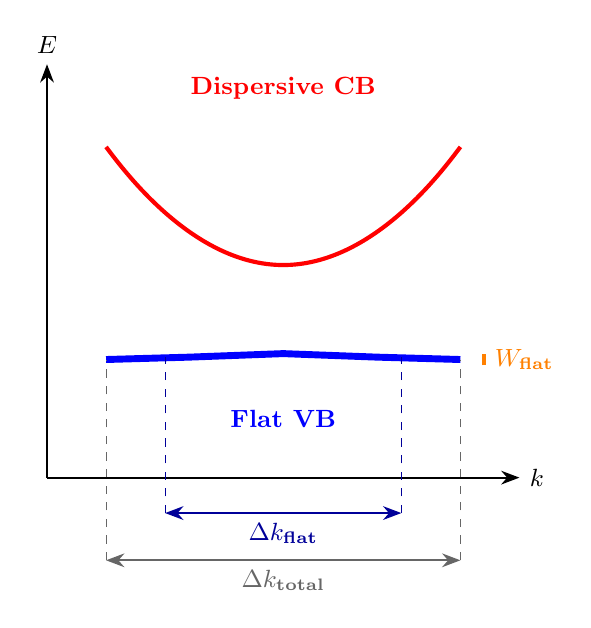
\begin{tikzpicture}[scale=1.5, >=Stealth, every node/.style={font=\small}]
    % Axes
    \draw[->, thick] (-2,-0.5) -- (2,-0.5) node[right] {\textcolor{black}{$k$}};
    \draw[->, thick] (-2,-0.5) -- (-2,3) node[above] {\textcolor{black}{$E$}};
    
    % Dispersive band
    \draw[thick, red, line width=1.5pt] 
      (-1.5,2.3) parabola bend (0,1.3) (1.5,2.3);
    \node[red] at (0,2.8) {\textbf{Dispersive CB}};
    
    % Flat band (with slight curvature to show W_flat)
    \draw[thick, blue, line width=2.5pt] 
      (-1.5,0.5) -- (-0.8,0.52) -- (0,0.55) -- (0.8,0.52) -- (1.5,0.5);
    \node[blue] at (0,0) {\textbf{Flat VB}};
    
    % Add vertical arrow showing flat bandwidth
    \draw[-, orange, very thick] (1.7,0.45) -- (1.7,0.55) 
      node[midway, right, orange] {\textbf{$W_{\text{flat}}$}};
      
    % Add k_flat region markers
    \draw[<->, thick, blue!60!black] (-1,-0.8) -- (1,-0.8) 
      node[midway, below] {\textbf{$\Delta k_{\text{flat}}$}};
    \draw[dashed, blue!60!black] (-1,-0.8) -- (-1,0.52);
    \draw[dashed, blue!60!black] (1,-0.8) -- (1,0.52);
    
    % Add k_total region markers
    \draw[<->, thick, black!60] (-1.5,-1.2) -- (1.5,-1.2) 
      node[midway, below] {\textbf{$\Delta k_{\text{total}}$}};
    \draw[dashed, black!60] (-1.5,-1.2) -- (-1.5,0.5);
    \draw[dashed, black!60] (1.5,-1.2) -- (1.5,0.5);
\end{tikzpicture}


\end{document}
